\documentclass{article}
\usepackage[margin=1in]{geometry}
\usepackage[linesnumbered,ruled,vlined]{algorithm2e}
\usepackage{amsfonts}
\usepackage{amsmath}
\usepackage{amssymb}
\usepackage{amsthm}
\usepackage{enumitem}
\usepackage{fancyhdr}
\usepackage{hyperref}
\usepackage{minted}
\usepackage{multicol}
\usepackage{pdfpages}
\usepackage{standalone}
\usepackage[many]{tcolorbox}
\usepackage{tikz-cd}
\usepackage{transparent}
\usepackage{xcolor}
% \tcbuselibrary{minted}

\author{Nathan Solomon}

\newcommand{\fig}[1]{
    \begin{center}
        \includegraphics[width=\textwidth]{#1}
    \end{center}
}

% Math commands
\renewcommand{\d}{\mathrm{d}}
\DeclareMathOperator{\id}{id}
\DeclareMathOperator{\im}{im}
\DeclareMathOperator{\proj}{proj}
\DeclareMathOperator{\Span}{span}
\DeclareMathOperator{\Tr}{Tr}
\DeclareMathOperator{\tr}{tr}
\DeclareMathOperator{\ad}{ad}
\DeclareMathOperator{\ord}{ord}
%%%%%%%%%%%%%%% \DeclareMathOperator{\sgn}{sgn}
\DeclareMathOperator{\Aut}{Aut}
\DeclareMathOperator{\Inn}{Inn}
\DeclareMathOperator{\Out}{Out}
\DeclareMathOperator{\stab}{stab}

\newcommand{\N}{\ensuremath{\mathbb{N}}}
\newcommand{\Z}{\ensuremath{\mathbb{Z}}}
\newcommand{\Q}{\ensuremath{\mathbb{Q}}}
\newcommand{\R}{\ensuremath{\mathbb{R}}}
\newcommand{\C}{\ensuremath{\mathbb{C}}}
\renewcommand{\H}{\ensuremath{\mathbb{H}}}
\newcommand{\F}{\ensuremath{\mathbb{F}}}

\newcommand{\E}{\ensuremath{\mathbb{E}}}
\renewcommand{\P}{\ensuremath{\mathbb{P}}}

\newcommand{\es}{\ensuremath{\varnothing}}
\newcommand{\inv}{\ensuremath{^{-1}}}
\newcommand{\eps}{\ensuremath{\varepsilon}}
\newcommand{\del}{\ensuremath{\partial}}
\renewcommand{\a}{\ensuremath{\alpha}}

\newcommand{\abs}[1]{\ensuremath{\left\lvert #1 \right\rvert}}
\newcommand{\norm}[1]{\ensuremath{\left\lVert #1\right\rVert}}
\newcommand{\mean}[1]{\ensuremath{\left\langle #1 \right\rangle}}
\newcommand{\floor}[1]{\ensuremath{\left\lfloor #1 \right\rfloor}}
\newcommand{\ceil}[1]{\ensuremath{\left\lceil #1 \right\rceil}}
\newcommand{\bra}[1]{\ensuremath{\left\langle #1 \right\rvert}}
\newcommand{\ket}[1]{\ensuremath{\left\lvert #1 \right\rangle}}
\newcommand{\braket}[2]{\ensuremath{\left.\left\langle #1\right\vert #2 \right\rangle}}

\newcommand{\catname}[1]{{\normalfont\textbf{#1}}}

\newcommand{\up}{\ensuremath{\uparrow}}
\newcommand{\down}{\ensuremath{\downarrow}}

% Custom environments
\newtheorem{thm}{Theorem}[section]

\definecolor{probBackgroundColor}{RGB}{250,240,240}
\definecolor{probAccentColor}{RGB}{140,40,0}
\newenvironment{prob}{
    \stepcounter{thm}
    \begin{tcolorbox}[
        boxrule=1pt,
        sharp corners,
        colback=probBackgroundColor,
        colframe=probAccentColor,
        borderline west={4pt}{0pt}{probAccentColor},
        breakable
    ]
    \color{probAccentColor}\textbf{Problem \thethm.} \color{black}
} {
    \end{tcolorbox}
}

\definecolor{exampleBackgroundColor}{RGB}{212,232,246}
\newenvironment{example}{
    \stepcounter{thm}
    \begin{tcolorbox}[
      boxrule=1pt,
      sharp corners,
      colback=exampleBackgroundColor,
      breakable
    ]
    \textbf{Example \thethm.}
} {
    \end{tcolorbox}
}

\definecolor{propBackgroundColor}{RGB}{255,245,220}
\definecolor{propAccentColor}{RGB}{150,100,0}
\newenvironment{prop}{
    \stepcounter{thm}
    \begin{tcolorbox}[
        boxrule=1pt,
        sharp corners,
        colback=propBackgroundColor,
        colframe=propAccentColor,
        breakable
    ]
    \color{propAccentColor}\textbf{Proposition \thethm. }\color{black}
} {
    \end{tcolorbox}
}

\definecolor{thmBackgroundColor}{RGB}{235,225,245}
\definecolor{thmAccentColor}{RGB}{50,0,100}
\renewenvironment{thm}{
    \stepcounter{thm}
    \begin{tcolorbox}[
        boxrule=1pt,
        sharp corners,
        colback=thmBackgroundColor,
        colframe=thmAccentColor,
        breakable
    ]
    \color{thmAccentColor}\textbf{Theorem \thethm. }\color{black}
} {
    \end{tcolorbox}
}

\definecolor{corBackgroundColor}{RGB}{240,250,250}
\definecolor{corAccentColor}{RGB}{50,100,100}
\newenvironment{cor}{
    \stepcounter{thm}
    \begin{tcolorbox}[
        enhanced,
        boxrule=0pt,
        frame hidden,
        sharp corners,
        colback=corBackgroundColor,
        borderline west={4pt}{0pt}{corAccentColor},
        breakable
    ]
    \color{corAccentColor}\textbf{Corollary \thethm. }\color{black}
} {
    \end{tcolorbox}
}

\definecolor{lemBackgroundColor}{RGB}{255,245,235}
\definecolor{lemAccentColor}{RGB}{250,125,0}
\newenvironment{lem}{
    \stepcounter{thm}
    \begin{tcolorbox}[
        enhanced,
        boxrule=0pt,
        frame hidden,
        sharp corners,
        colback=lemBackgroundColor,
        borderline west={4pt}{0pt}{lemAccentColor},
        breakable
    ]
    \color{lemAccentColor}\textbf{Lemma \thethm. }\color{black}
} {
    \end{tcolorbox}
}

\definecolor{proofBackgroundColor}{RGB}{255,255,255}
\definecolor{proofAccentColor}{RGB}{80,80,80}
\renewenvironment{proof}{
    \begin{tcolorbox}[
        enhanced,
        boxrule=1pt,
        sharp corners,
        colback=proofBackgroundColor,
        colframe=proofAccentColor,
        borderline west={4pt}{0pt}{proofAccentColor},
        breakable
    ]
    \color{proofAccentColor}\emph{\textbf{Proof. }}\color{black}
} {
    \qed \end{tcolorbox}
}

\definecolor{noteBackgroundColor}{RGB}{240,250,240}
\definecolor{noteAccentColor}{RGB}{30,130,30}
\newenvironment{note}{
    \begin{tcolorbox}[
        enhanced,
        boxrule=0pt,
        frame hidden,
        sharp corners,
        colback=noteBackgroundColor,
        borderline west={4pt}{0pt}{noteAccentColor},
        breakable
    ]
    \color{noteAccentColor}\textbf{Note. }\color{black}
} {
    \end{tcolorbox}
}


\fancyhf{}
\setlength{\headheight}{24pt}

\date{\today}
\title{Physics 245 Homework \#6}

\begin{document}
\maketitle

\begin{prob}
\end{prob}
\begin{enumerate}[label=(\alph*)]
    \item The given electric field is
        \[ E = E_0 \exp \left( - \frac{x^2+y^2}{w_0^2} \right) \exp \left( i (kz-\omega t + \phi) \right) \hat{x}, \]
        the Rabi frequency is
        \[ \Omega = \frac{d\cdot E}{\hbar}, \]
        and our formula for the Stark shift is
        \[ E_{Stark} = - \frac{\hbar \abs{\Omega}^2}{4 \delta}. \]
        Therefore the Stark shift on the atom is
        \[ E_{Stark} = - \frac{d^2 \abs{E}^2}{4 \delta \hbar} = - \frac{d^2 E_0^2}{4 \delta \hbar} \exp \left( -2 \cdot \frac{x^2 + y^2}{w_0^2} \right). \]
    \item Let $r = \sqrt{x^2+y^2}$, so $r$ is a unitless quantity representing the distance away from the center of the atom. The change in potential is equal to the Stark shift, and to model the new potential with a harmonic oscillator, we need to approximate $E_{Stark}$ to second order in $r$:
        \[ E_{Stark} = - \frac{d^2 E_0^2}{4 \delta \hbar} e^{-2r^2/w_0^2} \approx - \frac{d^2 E_0^2}{4 \delta \hbar} \left( 1 - \frac{2r^2}{w_0^2} \right).  \]
        The coefficient of $r^2$ in that expression is
        \[ \frac{V(r)}{r^2} = \frac{m\omega^2}{2} = \frac{d^2 E_0^2}{2 \delta \hbar w_0^2}. \]
        Now we can solve for the natural frequency:
        \[ \omega = \frac{d E_0}{w_0 \sqrt{m \hbar \delta}}. \]
    \item Using the relations
        \[ I = \frac{1}{2} c \varepsilon_0 \abs{E}^2 = c \varepsilon_0 E_0^2 \exp \left( -2 \cdot \frac{r^2}{w_0^2} \right)  \]
        for the intensity of the laser and
        \begin{align*}
            P &= \iint I \d A \\
              &= c \varepsilon_0 E_0^2 \int_{r=0}^\infty \int_{\theta=0}^{2\pi} \exp \left( -2 \cdot \frac{r^2}{w_0^2} \right) \left( r \d \theta \d r \right)  \\
              &= 2 \pi c \varepsilon_0 E_0^2 \int_{r=0}^\infty r \cdot \exp \left( -2 \cdot \frac{r^2}{w_0^2} \right) \d r  \\
              &= 2 \pi c \varepsilon_0 E_0^2 \cdot \frac{w_0^2}{4} \\
              &= \frac{\pi}{2} c \varepsilon_0 E_0^2 w_0^2 \\
        \end{align*}
        for the power of the laser, the (angular) frequency is
        \begin{align*}
        \omega &= \frac{d}{w_0 \sqrt{m \hbar \delta}}\cdot E_0 \\
               &= \frac{d}{w_0 \sqrt{m \hbar \delta}}\cdot P \sqrt{ \frac{2}{\pi c \varepsilon_0 w_0^2}} \\
               &= \frac{d}{w_0^2}\cdot \sqrt{ \frac{2P}{\pi c \varepsilon_0 m \hbar \delta}} \\
               &= \frac{e a_0}{(10 \mu m)^2}\cdot \sqrt{ \frac{2P}{\pi c \varepsilon_0 m \hbar (10 THz)}} \\
               &= \frac{4 \pi \varepsilon_0 \hbar^2}{m_e e^2} \cdot \frac{e }{(10 \mu m)^2}\cdot \sqrt{ \frac{2(100mW)}{\pi c \varepsilon_0 m_e \hbar (10 THz)}} \\
               &= \frac{4 \sqrt{2 \pi \varepsilon_0 \hbar^3}}{e \sqrt{m_e^3 c}} \cdot \frac{\sqrt{100 mW}}{(10^{-5}m)^2 \sqrt{10^{13} s^{-1}}} \\
               &= \frac{4 P \sqrt{2 \pi \varepsilon_0 \hbar^3}}{e \sqrt{m_e^3 c}} \cdot \frac{\sqrt{100mW}}{(10^{-5}m)^2 \sqrt{10^{13} s^{-1}}} \\
               &= 13.3962824 \text{ megahertz}.
        \end{align*}
    \item $\omega$ is an angular frequency, so I can multiply it by $\hbar$ to get an energy, then divide that to get a temperature (in Kelvin).
        \[ \frac{\hbar \omega}{k} = 0.00010232392 K \approx 0.1 mK. \]
        
\end{enumerate}

\bigskip
\begin{prob}
\end{prob}
\begin{enumerate}[label=(\alph*)]
    \item Using the notation from chapter 7 in Griffiths,
        \[ H = H^0 + \lambda H', \]
        where $H'=x^4$. Then the first order correction to $\psi_n$ is
        \[ \psi_n^1 := \sum_{m \neq n} \frac{\bra{\psi_m^0}\lambda H'\ket{\psi_n^0}}{E_n^0-E_m^0} \psi_m^0. \]
        See the jupyter notebook for the actual calculations of those corrections.
    \item The second order energy corrections are
        \[ E_n^2 = \sum_{m \neq n} \frac{\abs{\bra{\psi_m^0} \lambda H' \ket{\psi_n^0}}^2}{E_n^0-E_m^0}. \]
        Once again, see the jupyter notebook at the end of this doc for the actual calculations.
    \item See jupyter notebook for calculations. I experimented with changing the value of $n_{max}$ and found that increasing $n_{max}$ makes all of my predicted energies more accurate. By ``predicted energies", I mean the unperturbed energies plus the first and second order corrections.
\end{enumerate}


\bigskip
\begin{prob}
\end{prob}
\textbf{For parts (a) through (c)}, see the jupyter notebook.
\par
\textbf{For part (d):}
\[ \begin{bmatrix}
    a_1 \\
    b_1
\end{bmatrix} \otimes \begin{bmatrix}
    a_2 \\
    b_2
\end{bmatrix} \otimes \begin{bmatrix}
    a_3 \\
    b_3
\end{bmatrix} = \begin{bmatrix}
    a_1 a_2 a_3 \\
    a_1 a_2 b_3 \\
    a_1 b_2 a_3 \\
    a_1 b_2 b_3 \\
    b_1 a_2 a_3 \\
    b_1 a_2 b_3 \\
    b_1 b_2 a_3 \\
    b_1 b_2 b_3
\end{bmatrix}. \]
\par
\textbf{For part (e):}
\par
The total state vector is
\[ \frac{1}{\sqrt{3}} \begin{bmatrix}
    a_1 \\
    a_1 \\
    0 \\
    a_1 \\
    b_1 \\
    b_1 \\
    0 \\
    b_1
\end{bmatrix}. \]
\par
The expectation value of $\sigma_x$ on the qubit is
\begin{align*}
    (\ket{\psi} \otimes \ket{\phi})^\dag (\sigma_x \otimes I) (\ket{\psi} \otimes \ket{\phi}) &= (\ket{\psi} \otimes \ket{\phi})^\dag (\sigma_x \ket{\psi} \otimes I \ket{\phi}) \\
                                                                                          &= (\bra{\psi} \otimes \bra{\phi}) (\sigma_x \ket{\psi} \otimes I \ket{\phi}) \\
                                                                                          &= \bra{\psi} \sigma_x \ket{\psi} \cdot \bra{\phi} I \ket{\phi} \\
                                                                                          &= \bra{\psi} \sigma_x \ket{\psi} \\
                                                                                          &= a_1^2 - b_1^2.
\end{align*}
Using that same trick with the tensor products, the expectation of $N$ on the harmonic oscillator, which is the expectation value $\mean{I \otimes N} = (\ket{\psi} \otimes \ket{\phi})^\dag (I \otimes N) (\ket{\psi} \otimes \ket{\phi})$, can be rewritten as $\bra{\phi} N \ket{\phi}$:
\begin{align*}
    \mean{I \otimes N} &= \bra{\phi} N \ket{\phi} \\
                       &= \left( \frac{1}{\sqrt{3}} \right)^2 \left( 0 + 1 + 3 \right) \\
                       &= \frac{4}{3}.
\end{align*}
In the composite statevector, the coefficient of $\ket{1} \otimes \ket{3}$ is $b_1/\sqrt{3}$, so the probabilitiy of finding the qubit in state $\ket{1}$ and the harmonic oscillator in state $\ket{3}$ is $\abs{b_1}^2/3$.

\bigskip
\begin{prob}
\end{prob}
See the jupyter notebook.

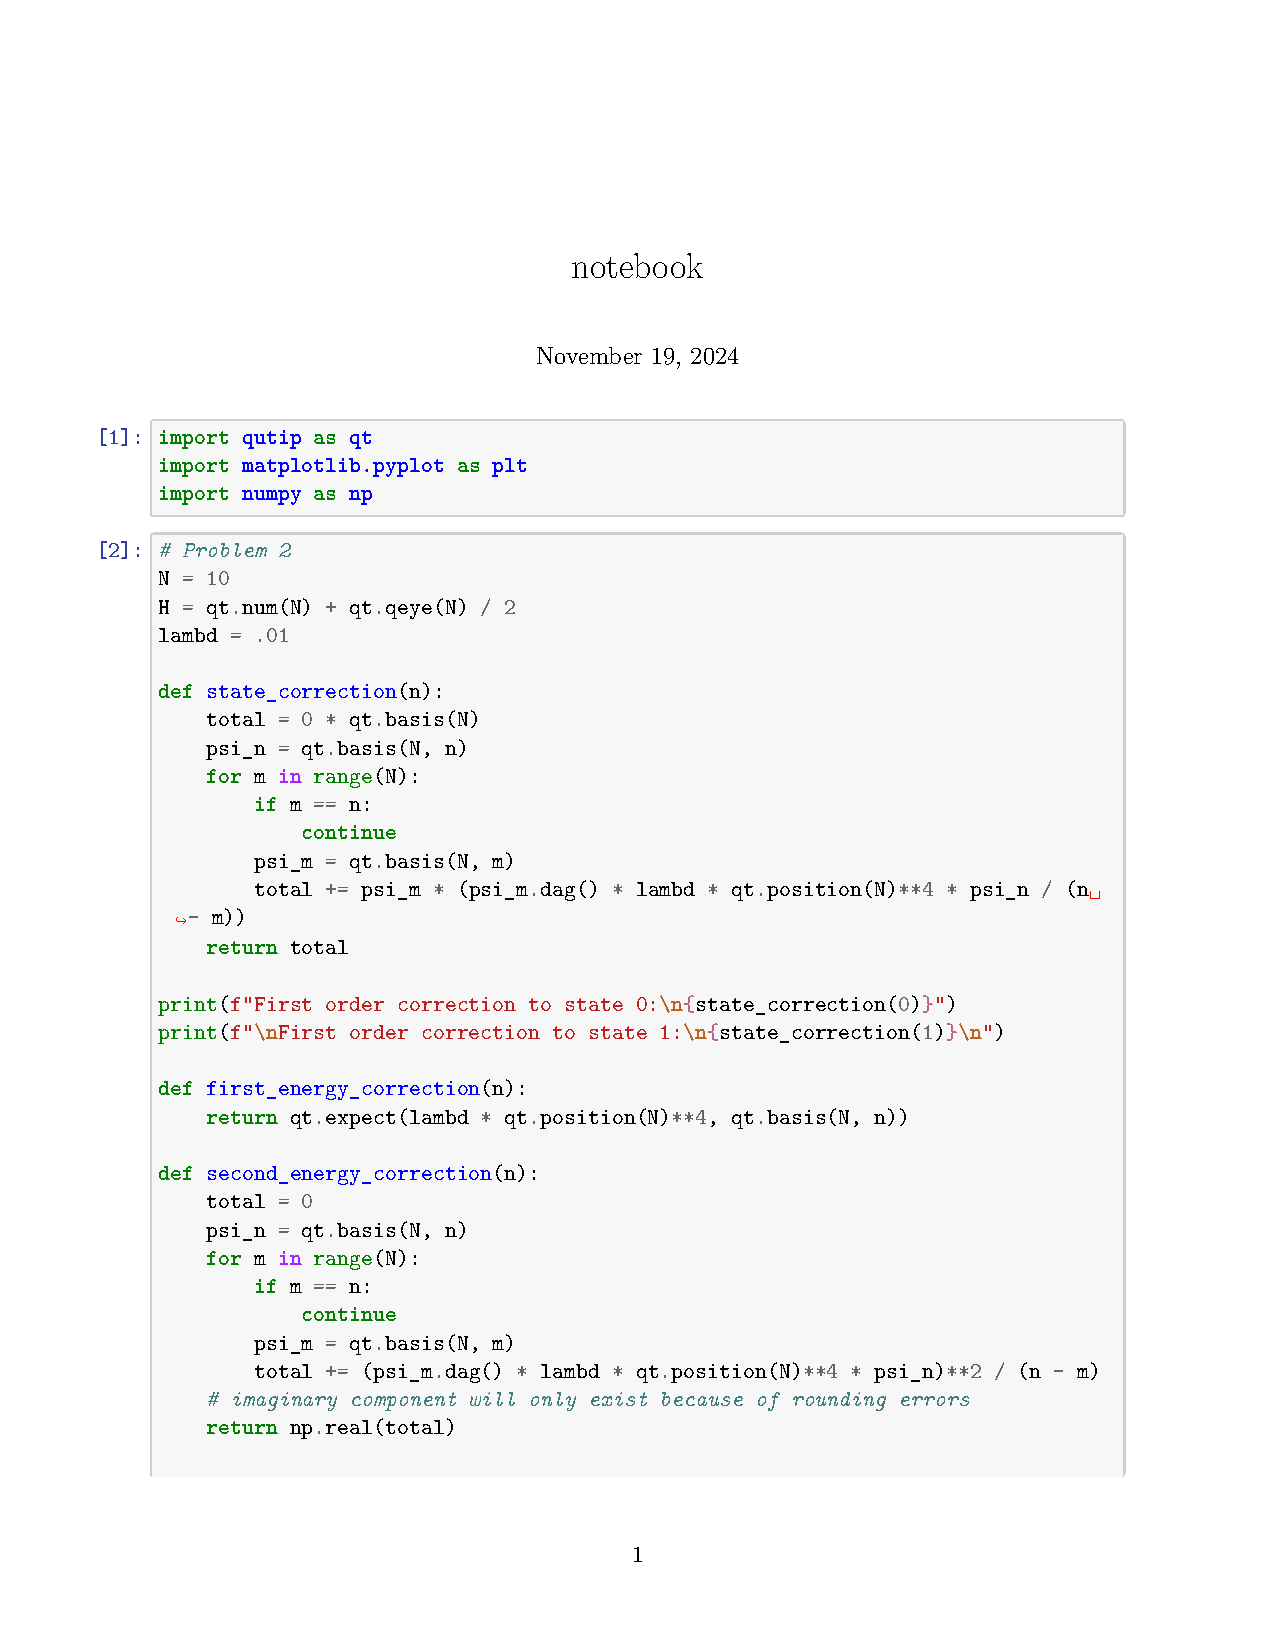
\includepdf[pages=-]{notebook.pdf}
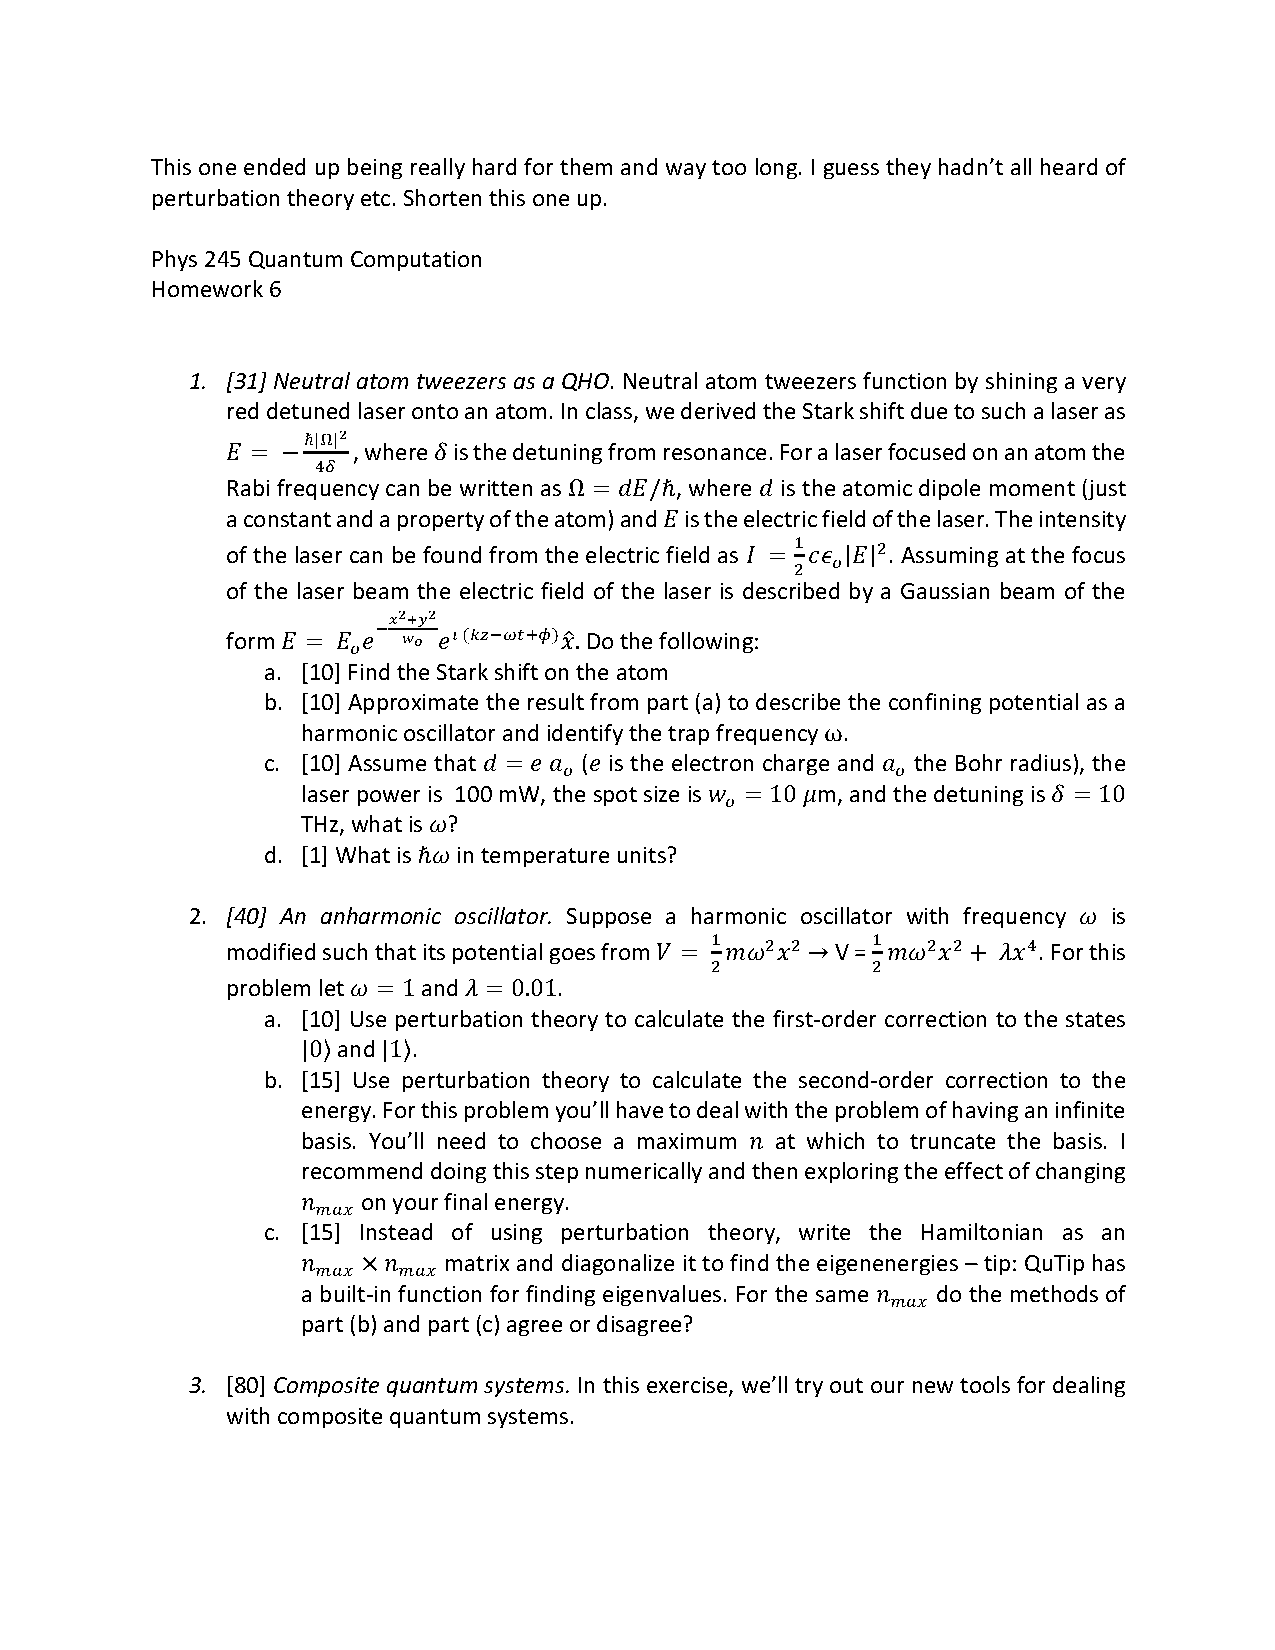
\includepdf[pages=-]{assignment.pdf}

\end{document}
